\section[Diagramme d'état et machines réelles]{Diagramme d'état \texorpdfstring{$(\log P,h)$}{(log P,h)} d'un fluide et fonctionnement de machines thermiques réelles}

    \subsection{Lecture du diagramme \texorpdfstring{$(\log P,h)$}{(log P,h)} d'un fluide pur}

        On veut caractériser l'état d'un fluide pur déterminé par la donnée de deux grandeurs intensives :
        \begin{itemize}
            \item $(P,v_m)$ [Clapeyron];
            \item $(P,h)$;
            \item $(T,s)$;
            \item $(h,s)$ [Mollier].
        \end{itemize}

        \subsubsection{Partition du plan $(\log P,h)$}

            \begin{figure}
                \centering
                \tikzsetnextfilename{lecture_diagramme_log_p_h_fluide_pur}
                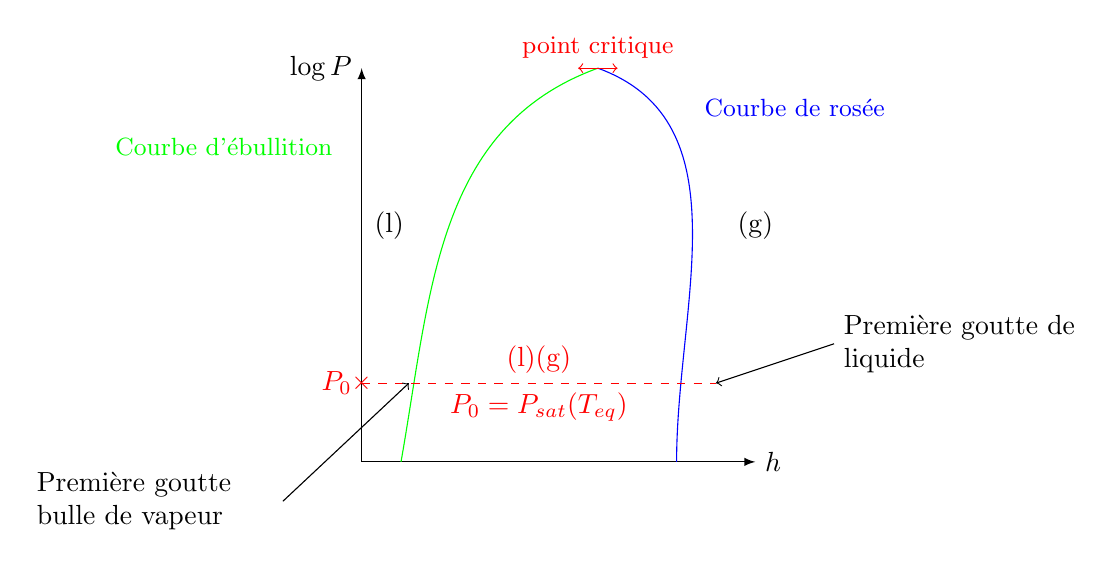
\begin{tikzpicture}[scale=1]  
                    % \helpgrid{3}{3}
                    
                    \draw[-latex] (0,0)--++(5,0) node [right] {$h$};
                    \draw[-latex] (0,0)--++(0,5) node [left] {$\log P$};
                    \node [text=red] at (0,1) {\small$\times$};
                    \node [text=red] at (0,1) [left] {$P_0$};

                    \draw [draw=green] (0.5,0) to[out=80,in=200] (3,5);
                    \draw [draw=blue] (3,5) to[out=-20,in=90] (4,0);

                    \node at (0.35,3) {(l)};
                    \node at (5,3) {(g)};

                    \draw[<->,draw=red,text=red] (2.75,5)--++(0.5,0) node [above,midway] {\small point critique};
                    \node[text=blue] at (5.5,4.5) {\small Courbe de rosée};
                    \node[text=green] at (-1.75,4) {\small Courbe d'ébullition};
                    \draw[dashed,draw=red,text=red] (0,1) -- (4.5,1) node [below, midway] {$P_0=P_{\text{sat}}(T_{\text{eq}})$} node [above, midway] {(l)$\leftrightarrows$(g)};
                    \draw [<-] (4.5,1) to (6,1.5) node [right,text width=3cm] {Première goutte de liquide};
                    \draw [<-] (0.6,1) to (-1,-0.5) node [left,text width=3cm] {Première goutte bulle de vapeur};
                \end{tikzpicture}
                \caption{Partition du plan $(\log P,h)$.}    
                \label{fig:lecture_diagramme_log_p_h_fluide_pur}
            \end{figure}

            On donne la partition du plan $(\log P,h)$ à la Figure~\ref{fig:lecture_diagramme_log_p_h_fluide_pur}. La courbe d'ébullition jointe avec la courbe de rosée s'appelle la \textbf{courbe de saturation}. On note $x$ le titre massique vapeur : pour une masse $m$ de fluide donnée, on a 
            \begin{equation}
                \boxed{
                    x\coloneqq\frac{m_{\text{gaz}}}{m},\qquad x_{l}=1-x.
                }
            \end{equation}

            Pour le calculer, on considère la situation de la Figure~\ref{fig:titre_vapeur_theoreme_moments_titre_massique_vapeur}.
            
            \begin{figure}
                \centering
                \tikzsetnextfilename{titre_vapeur_theoreme_moments_titre_massique_vapeur}
                \begin{tikzpicture}[scale=1]  
                    % \helpgrid{3}{3}
                    
                    \draw[-latex] (0,0)--++(5,0) node [right] {$h$};
                    \draw[-latex] (0,0)--++(0,5) node [left] {$\log P$};
                    \node [text=red] at (0,3) {\small$\times$};
                    \node [text=red] at (0,3) [left] {$P_0$};
                    \draw[dashed,draw=red,text=red] (0,3) -- (4.2,3);

                    \draw [draw=green] (0.5,0) to[out=80,in=200] (3,5);
                    \draw [draw=blue] (3,5) to[out=-20,in=90] (4,0);

                    
                    \node[text=red] at (1.1,3) {$\bullet$};
                    \node[text=red] at (4.2,3) {$\bullet$};
                    \node[text=red] at (1.1,3) [above] {L};
                    \node[text=red] at (4.2,3) [above] {G};
                    \node at (2.5,3) {$\bullet$};
                    \node at (2.5,3) [above] {M};
                    \draw [dashed] (2.5,3) --++(0,-3) node [below] {$h$};
                    \draw [dashed, draw=red,text=red] (1.1,3) --++(0,-3) node [below] {$h_l$};
                    \draw [dashed, draw=red,text=red] (4.2,3) --++(0,-3) node [below] {$h_g$};
                    \draw[stealth-stealth, draw=red,text=red] (1.1,-1)--(4.2,-1) node [below, midway] {$\Delta h_{\text{vap}}$};


                \end{tikzpicture}
                \caption{Théorème des moments pour le titre massique en vapeur.}    
                \label{fig:titre_vapeur_theoreme_moments_titre_massique_vapeur}
            \end{figure}

            L'enthalpie $H$ de la masse $m$ représenté par le point $M$ est 
            \begin{equation}
                H(T,m,x)= m_g h_g(T_{\text{eq}})+m_l h_l(T_{\text{eq}})=m\left[x h_g+(1-x)h_l\right],
            \end{equation}
            en utilisant le fait que l'enthalpie est une fonction extensive. Ainsi,
            \begin{equation}
                \boxed{
                    h(T_{\text{eq}},x)=h(P_0,x)=xh_g(P_0)+(1-x)h_l(P_0).
                }
            \end{equation}

            Ainsi, en $M$, on a 
            \begin{equation}
                \boxed{
                    x=\frac{h-h_l}{h_g-h_l}=\frac{LM}{LG}.
                }
            \end{equation}
            C'est le \textbf{théorème des moments}. Les courbes isotitres sont représentées à la Figure~\ref{fig:titre_vapeur_theoreme_moments_titre_massique_vapeur_isotitres}.
            \begin{figure}
                \centering
                \tikzsetnextfilename{titre_vapeur_theoreme_moments_titre_massique_vapeur_isotitres}
                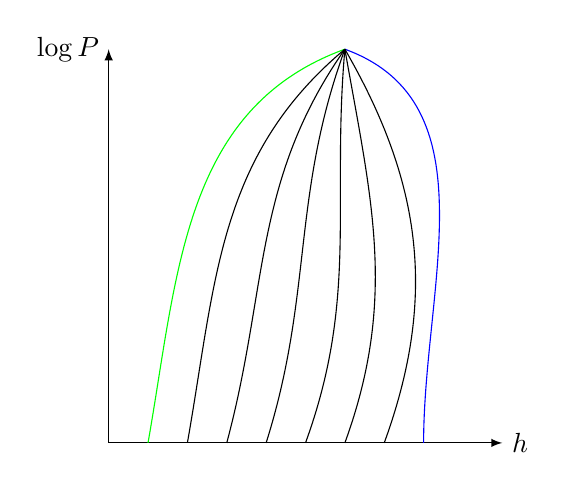
\begin{tikzpicture}[scale=1]  
                    % \helpgrid{3}{3}
                    
                    \draw[-latex] (0,0)--++(5,0) node [right] {$h$};
                    \draw[-latex] (0,0)--++(0,5) node [left] {$\log P$};

                    \draw  [draw=green] (0.5,0) to[out=80,in=200] (3,5);
                    \draw  [draw=blue] (3,5) to[out=-20,in=90] (4,0);

                    \draw  (1,0)  to [out=80, in=220] (3,5);
                    \draw  (1.5,0) to [out=75, in=235] (3,5);
                    \draw  (2,0) to [out=72.5, in=250] (3,5);
                    \draw  (2.5,0) to [out=70, in=265] (3,5);
                    \draw  (3,0) to [out=70, in=280] (3,5);
                    \draw  (3.5,0) to [out=70, in=300] (3,5);

                \end{tikzpicture}
                \caption{Isotitres massique en vapeur pour le diagramme $(\log P,h)$.}    
                \label{fig:titre_vapeur_theoreme_moments_titre_massique_vapeur_isotitres}
            \end{figure}

        \subsubsection{Les différents réseaux de courbes}

            \begin{itemize}
                \item Isobares : horizontales (\si[]{\bar});
                \item Isenthalpiques : verticales (\si[]{\kilo\joule\per\kilogram});
                \item Isothermes (\si[]{\celsius}) : 
                \begin{itemize}
                    \item horizontales dans la zone ($(l)\leftrightarrows (g)$);
                    \item environ verticales dans la zone (l), car
                    \begin{equation}
                        \d h_l=c\d T,
                    \end{equation}
                    donc $h_l(T)$;
                    \item environ verticales à basse pression et pas trop près de la courbe de saturation car, dans ce cas, c'est environ un gaz parfait et la deuxième loi de Joule pour les gaz parfaits implique $h_g(T)$.
                \end{itemize}
                \item isochores : courbes croissantes (avec rupture de pente sur la courbe de rosée) \si[]{\metre\cubed\per\kilogram};
                \item isentropiques : courbes croissantes sans rupture de pente \si[]{\kilo\joule\per\kilogram\per\kelvin}, environ verticales dans la zone (l) car 
                \begin{equation}
                    s_l=C_{p,m}\ln\left(\frac{T}{T_0}\right)+s_0.
                \end{equation}
            \end{itemize}

        \subsubsection{Intérêt pour les écoulements permanents}

            Un fluide en écoulement permanent a une variation d'enthalpie massique égale à 
            \begin{equation}
                \Delta h=\omega_i+q.
            \end{equation}
            \begin{example}
                Pour un compresseur isentropique, on a $\Delta h=\omega_i$ : la transition suit une courbe isenthalpique croissante car $\omega_i>0$.
            \end{example}
            \begin{example}
                Pour une chaudière, on a $\Delta h=q$ : la transition suit une transition isobare (courbe horizontale) de gauche à droite car $q>0$.
            \end{example}

    \subsection{Exemple : cycle moteur à vapeur d'une centrale électrique}

        La combustion du carbone ou la fission nucléaire introduit un transfert thermique (chaudière) qui crée un travail mécanique (turbine). Le \textbf{cycle de Rankine} est présenté à la Figure~\ref{fig:cycle_rankine_moteur_vapeur_centrale_electrique}.

        \begin{figure}
            \centering
            \tikzsetnextfilename{cycle_rankine_moteur_vapeur_centrale_electrique}
            \begin{tikzpicture}[scale=0.75,decoration={
                markings,
                mark=at position 0.5 with {\arrow{>}}}
                ] ]  
                % \helpgrid{3}{3}
                
                \coordinate (A) at (0,0);
                \coordinate (A1) at (0,1);
                \draw[smooth] (0,2) circle (1) node {pompe};
                \coordinate (A2) at (0,3);
                \coordinate (B) at (0,4);
                \draw[postaction={decorate}] (A)--(A1);
                \draw[postaction={decorate}] (A2)--(B);
                \coordinate (B1) at (1,4);
                \draw (1,3.75) rectangle (3,4.25) node[midway] {\small chaudière};
                \coordinate (B2) at (3,4);
                \coordinate (C) at (4,4);
                \draw[postaction={decorate}] (B)--(B1);
                \draw[postaction={decorate}] (B2)--(C);
                \coordinate (C1) at (4,2.28);
                \node [trapezium, draw] (t) at (4,2){turbine};
                \coordinate (C2) at (4,1.73);
                \coordinate (D) at (4,0);
                \draw[postaction={decorate}] (C)--(C1);
                \draw[postaction={decorate}] (C2)--(D);
                \coordinate (D1) at (3,0);
                \draw[smooth] (2,0) circle (1);
                \coordinate (D2) at (1,0);
                \draw (D1) -- (D2);
                \node at (2,-1.75) {\small condenseur};
                \draw[postaction={decorate}] (D)--(D1);
                \draw[postaction={decorate}] (D2)--(A);

                \draw[-stealth] (-3,1) --++ (0,2) node [left, midway, text width=2.5cm] {compression isentropique};
                \draw[-stealth] (7,3) --++ (0,-2) node [right, midway, text width=2.5cm] {détente\\isentropique}; 
                \draw [-stealth] (1,4.5) --++ (2,0) node [above, midway,  text width=2.5cm] {chauffage isobare};
                \draw [-stealth] (3,-2.5) --++ (-2,0) node [below, midway,  text width=2.5cm] {condensation totale isobare};

                \draw [-stealth, double, draw=green, text=green] (2,3.25)--++(0,0.5) node [right, midway] {$q_c>0$};
                \draw [-stealth, double, draw=green, text=green] (2,-1)--++(0,-0.5) node [right, midway] {$q_f<0$};
                \draw [-stealth, double, draw=red, text=red] (-2,2)--++(0.5,0) node [below, midway] {$w_p>0$};
                \draw [-stealth, double, draw=red, text=red] (5.5,2)--++(0.5,0) node [below, midway] {$w_t<0$};

                \draw [<-] (0,0)--++(-1,-1) node [below left, text width=4cm] {liquide juste saturant $T_1,P_1=P_{\text{sat}}(T_1)$} node [midway, above] {1};
                \draw [<-] (0,4)--++(-1,1) node [above left, text width=4cm] {liquide à\\$P_2>P_1$,$T_2\approx T_1$} node [midway, above] {2};
                \draw [<-] (4,4)--++(1,1) node [above right, text width=4cm] {Vapeur sèche\\$T3>T_{\text{cb}}(P_2),P_2$} node [midway, above] {3};
                \draw [<-] (4,0)--++(1,-1) node [below right, text width=4.5cm] {Système diphasé (l+g),\\$x_4,T_4=T_1$,\\$P_4=P_{\text{sat}}(T_1)=P_1$} node [midway, above] {4};
            \end{tikzpicture}
            \caption{Cycle de Rankine pour une centrale électrique.}    
            \label{fig:cycle_rankine_moteur_vapeur_centrale_electrique}
        \end{figure}

        On donne $P_1=P_4=0,2~\si[]{\bar}$, $P_2=P_3=10~\si[]{\bar}$, $T_3=340~\si[]{\celsius}$. L'eau est en écoulement permanent donc 
        \begin{equation}
            \Delta h+\Delta\left(\frac{v^{2}}{2}+gz\right)=\omega_i+q.
        \end{equation}
        On a 
        \begin{equation}
            \begin{aligned}
                \Delta h\sim& 100~\si[]{\kilo\joule\per\kg},\\
                \Delta e_c=\frac{v^{2}}{2}-0\sim& 1000~\si[]{\kilo\joule\per\kg},\\
                v\sim&1400~\si[]{\metre\per\second},\\
                \Delta(gz)\sim& 10\Delta z,\\
                \Delta z\sim&100~\si[]{\kilo\metre}.
            \end{aligned}
        \end{equation}
        Ainsi, $\Delta e_c\ll\Delta h$ et $\Delta(gz)\ll\Delta h$. Ainsi,
        \begin{equation}
            \boxed{
                \Delta h=\omega_i+q.
            }
        \end{equation}

        \begin{itemize}
            \item Pompe : $\omega_p=h_2-h_1, s_2=s_1$;
            \item Chaudière : $q_c=h_3-h_2, s_3-s_2>s_e>0$, et $s_e\neq q_c/T_3$ (car il n'y a pas qu'un changement d'état);
            \item Turbine : $\omega_t=h_4-h_3,s_4=s_3$;
            \item $q_f=h_1-h_4,s_1-s_4=s_e+s_c=s_e=q_f/T_1$ car c'est un changement d'état.
        \end{itemize}

        Le rendement est donné par 
        \begin{align}
            \eta
            &=
            \left\lvert\frac{\text{grandeur désirée}}{\text{grandeur coûteuse}}\right\rvert,\\
            &=\frac{-\omega_t-\omega_p}{q_c}.
        \end{align}

        On a typiquement
        \begin{equation}
            \begin{aligned}
                \omega_p\sim&15~\si[]{\kilo\joule\per\kilogram},\\
                q_c\sim&2800~\si[]{\kilo\joule\per\kilogram},\\
                \omega_t\sim&-750\si[]{\kilo\joule\per\kilogram},\\
                q_f\sim-2000~\si[]{\kilo\joule\per\kilogram}.
            \end{aligned}
        \end{equation}
        Donc 
        \begin{equation}
            \boxed{
                \eta\approx\frac{-\omega_t}{q_c}=\approx 0.26.
            }
        \end{equation}

        Notons que pour un moteur de Carnot entre $T_1$ et $T_3$ ($60~\si[]{\celsius}$ et $340~\si[]{\celsius}$), on a (température en $\si[]{\kelvin}$)
        \begin{equation}
            \eta_c=1-\frac{T_f}{T_c}=0.46.
        \end{equation}

    \subsection{Réfrigérateur à compresseur}
        
        Le cycle est donné à la Figure~\ref{fig:cycle_refrigerateur_a_compresseur}.

        \begin{figure}
            \centering
            \tikzsetnextfilename{cycle_refrigerateur_a_compresseur}
            \begin{tikzpicture}[scale=0.75,decoration={
                markings,
                mark=at position 0.5 with {\arrow{>}}}
                ] ]  
                % \helpgrid{3}{3}
                
                \coordinate (A) at (0,0);
                \coordinate (A1) at (0,1.73);
                \node [trapezium, draw] (t) at (0,2){compresseur};
                \coordinate (A2) at (0,2.28);
                \coordinate (B) at (0,4);
                \draw[postaction={decorate}] (A)--(A1);
                \draw[postaction={decorate}] (A2)--(B);
                \coordinate (B1) at (1,4);
                \draw (1,3.75) rectangle (3,4.25) node[midway] {\small condenseur};
                \coordinate (B2) at (3,4);
                \coordinate (C) at (4,4);
                \draw[postaction={decorate}] (B)--(B1);
                \draw[postaction={decorate}] (B2)--(C);
                \coordinate (C1) at (4,3);
                \draw (4.5,3)--(3.5,1)--(4.5,1)--(3.5,3)--(4.5,3);
                \node at (5.2,2) {détendeur};
                \coordinate (C2) at (4,1);
                \coordinate (D) at (4,0);
                \draw[postaction={decorate}] (C)--(C1);
                \draw[postaction={decorate}] (C2)--(D);
                \coordinate (D1) at (3,0);
                \coordinate (D2) at (1,0);
                \draw (1,-0.25) rectangle (3,0.25) node[midway] {\footnotesize évaporateur};
                \draw[postaction={decorate}] (D)--(D1);
                \draw[postaction={decorate}] (D2)--(A);

                \draw[-stealth] (-3,1) --++ (0,2) node [left, midway, text width=2.5cm] {compression isentropique};
                \draw[-stealth] (7,3) --++ (0,-2) node [right, midway, text width=2.5cm] {isenthalpique}; 
                \draw [-stealth] (1,4.5) --++ (2,0) node [above, midway,  text width=2.5cm] {isobare};
                \draw [-stealth] (3,-1.5) --++ (-2,0) node [below, midway,  text width=2.5cm] {vaporisation\\complète};

                \node [text=green] at (2,3.5) {$\downarrow\left\lvert q_c\right\rvert$};
                \draw [-stealth, double, draw=green, text=green] (2,-0.75)--++(0,0.5) node [right, midway] {$q_f$};
                \draw [-stealth, double, draw=red, text=red] (-2.5,2)--++(0.5,0) node [below, midway] {$w_c>0$};

                \draw [<-] (0,0)--++(-1,-1) node [below left, text width=4cm] {vapeur saturante\\ $T_1=253~\si[]{\kelvin},P_1$} node [midway, above] {1};
                \draw [<-] (0,4)--++(-1,1) node [above left, text width=4cm] {vapeur sèche\\$P_2>P_1,T_2>T_1$} node [midway, above] {2};
                \draw [<-] (4,4)--++(1,1) node [above right, text width=4cm] {liquide saturant\\$P_3=P_2=8~\si[]{\bar},T_3$} node [midway, above] {3};
                \draw [<-] (4,0)--++(1,-1) node [below right, text width=4.5cm] {Mélange (l+g)\\$x_4$, $P_4=P_1$\\$T_4=T_1$} node [midway, above] {4};
            \end{tikzpicture}
            \caption{Cycle d'un réfrigérateur à compresseur.}    
            \label{fig:cycle_refrigerateur_a_compresseur}
        \end{figure}
        
        On donne $P_1=1,3~\si[]{\bar}$ et $T_3=31~\si[]{\celsius}$. Le premier principe donne (données dans une annexe) :
        \begin{itemize}
            \item Compression : $\omega_c=h_2-h_1=40~\si[]{\kilo\joule\per\kilogram}$;
            \item Condenseur : $q_c=-180~\si[]{\kilo\joule\per\kilogram}$;
            \item Détendeur : $h_4=h_3$;
            \item Évaporateur : $q_f=h_1-h_4=140~\si[]{\kilo\joule\per\kilogram}$.
        \end{itemize}

        Le deuxième principe donne :
        \begin{itemize}
            \item Compression : $s_2=s_1$;
            \item Condenseur : $s_3-s_2=s_{\text{ech}}+s_{\text{cr}}>q_c/T_3$;
            \item Détendeur : $s_4-s_3=0+s_{\text{cr}}>0$ donc $s_4>s_3$;
            \item Évaporateur : $s_4-s_1\geqslant q_f/T_c$.
        \end{itemize}

        Le coefficient de performance est 
        \begin{equation}
            \text{COP}=\frac{q_f}{\omega_c}\approx3.5.
        \end{equation}

        Le cycle de Carnot donne 
        \begin{equation}
            \text{COP}=\frac{T_f}{T_c-T_f}=5.6,
        \end{equation}
        avec $T_c=25~\si[]{\celsius}$ et $T_f=T_1=-20~\si{\celsius}$.